% !TEX root = ../example_paper.tex

\section{Hardware}
\subsection{Model}
\label{sec:hardware}
Kolesá a ozubené koliečko pre hriadeľ motora boli vytlačené v 3D tlačiarni s resinovou náplňou \textbf{FabPro 1000 Resin Cartridge Tough BLK}. Na obrázkoch \ref{fig:gear} a \ref{fig:wheel_w_gear} môžeme vidieť návrhy ozubeého koliečka pre hriadeľ a kolesa. 

\begin{figure}[!htbp]
        \centering
        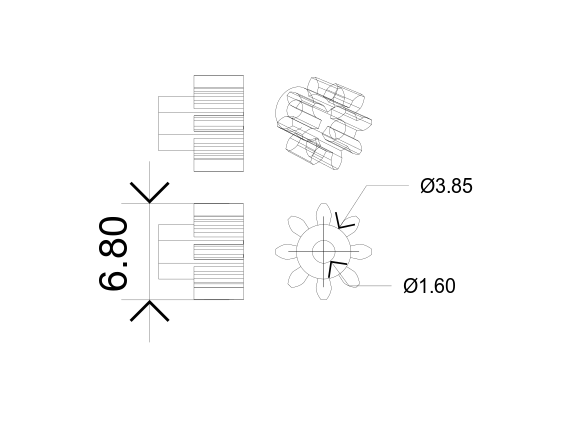
\includegraphics[scale=0.8]{includes/images/motor_gear.png}
        \caption{Užívateľské rozhranie s označenými komponentami}
        \label{fig:gear}
\end{figure}

\begin{figure}[!htbp]
        \centering
        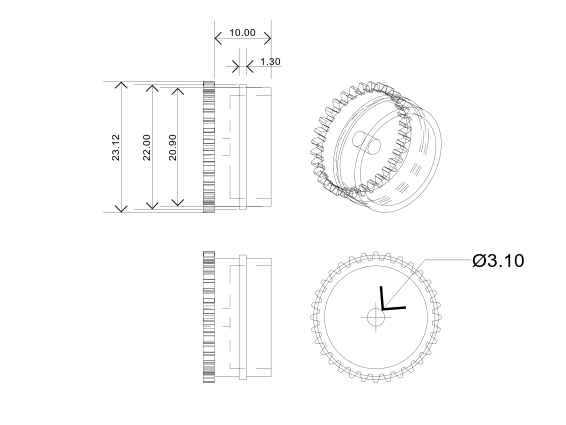
\includegraphics[scale=0.8]{includes/images/wheel_w_gear_2_blueprint.png}
        \caption{Koleso s ozubenými kolesami}
        \label{fig:wheel_w_gear}
\end{figure}
\newpage
\subsection{Motory}
Použité motory boli vybrané s ohľadom na ich výkonnosť a spoľahlivosť. Nižšie uvádzame detaily o týchto motoroch \ref{fig:motor}:

\begin{figure}[!htbp]
        \centering
        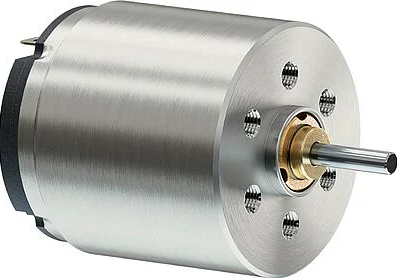
\includegraphics[scale=0.8]{includes/images/faulhaber.png}
        \caption{DC Mikromotor Faulhaber 1717T003SR}
        \label{fig:motor}
\end{figure}

\begin{itemize}
  \item Model: Faulhaber 1717 T 
  \item Typ: 003 SR
  \item Max. točivý moment: 5.35 mNm
  \item Max. rýchlosť: 11000 rpm
  \item Odkaz na technický list: \href{https://www.faulhaber.com/fileadmin/Import/Media/EN_1717_SR_DFF.pdf}{Technický list motora}
\end{itemize}

\subsection{Enkódery}
Na monitorovanie polohy a otáčok motorov sme použili enkódery. Nižšie sú uvedené informácie o použitých enkóderoch \ref{fig:encoder}:

\begin{figure}[!htbp]
        \centering
        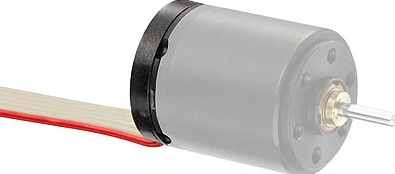
\includegraphics[scale=0.8]{includes/images/encoder.png}
        \caption{Enkóder IEH2-4096}
        \label{fig:encoder}
\end{figure}

\begin{itemize}
  \item Model: IEH2-4096
  \item Rozlíšenie: 4096
  \item Kanály: 2
  \item Odkaz na technický list: \href{https://www.faulhaber.com/fileadmin/Import/Media/EN_IEH2-4096_DFF.pdf}{Technický list enkódera}
\end{itemize}
Náklady na tieto motory so zabudovanýnmi enkódermi boli hradené školou vďaka finančnému príspevku od docenta Andreja Babinca.

\subsection{Gyroskop}

Na sledovanie orientácie a pohybu robota sme implementovali gyroskop. Ďalej sú uvedené podrobnosti o použitom gyroskopu \ref{fig:gyro}:
\begin{figure}[!htbp]
        \centering
        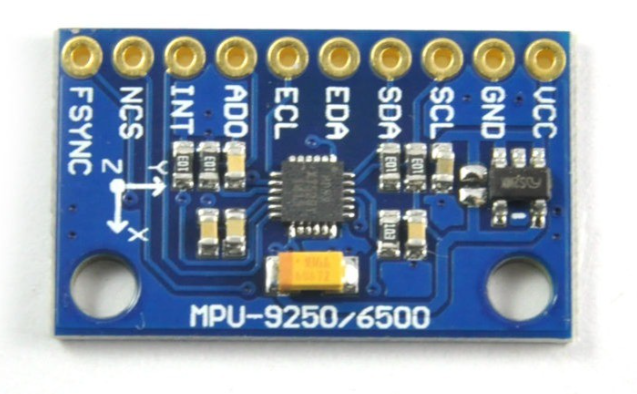
\includegraphics[scale=0.8]{includes/images/mpu9205.png}
        \caption{Gyroskop MPU9250}
        \label{fig:gyro}
\end{figure}
\begin{itemize}
  \item Model: MPU9250
  \item Typ: Gyroskop a akcelerometer
  \item Komunikácia: I2C, SPI
  \item Odkaz na technický list: \href{https://www.invensense.com/products/motion-tracking/9-axis/mpu-9250/}{MPU9250 Technical Datasheet}
\end{itemize}
\subsection{ToF}
Ako vzdialenostný senzor sme zvolili VL53L1X. Je to Time-of-Flight (doba trvania letu) laserový merací modul poskytujúci presné meranie vzdialenosti bez ohľadu na farbu alebo odrazivosť cieľa.

Tento kompaktný modul, ktorý môžeme vidieť na obrázku  \ref{fig:vl53l1x} dokáže spoľahlivo a rýchlo merať vzdialenosť až do 400cm s frekvecnciou do 50Hz. Jeho zorné pole je štandardne 27°, avšak je možnosť zmenšiť ho podľa potreby. Okrem pinov na napájanie a komunikáciu, taktiež obsahuje aj pin na prerušenie a pin na shutdown (vyradenie). Komunikácia so senzorom prebieha prostredníctvom protokolu $I^2 C$.

\begin{figure}[!htpb]
    \centering
    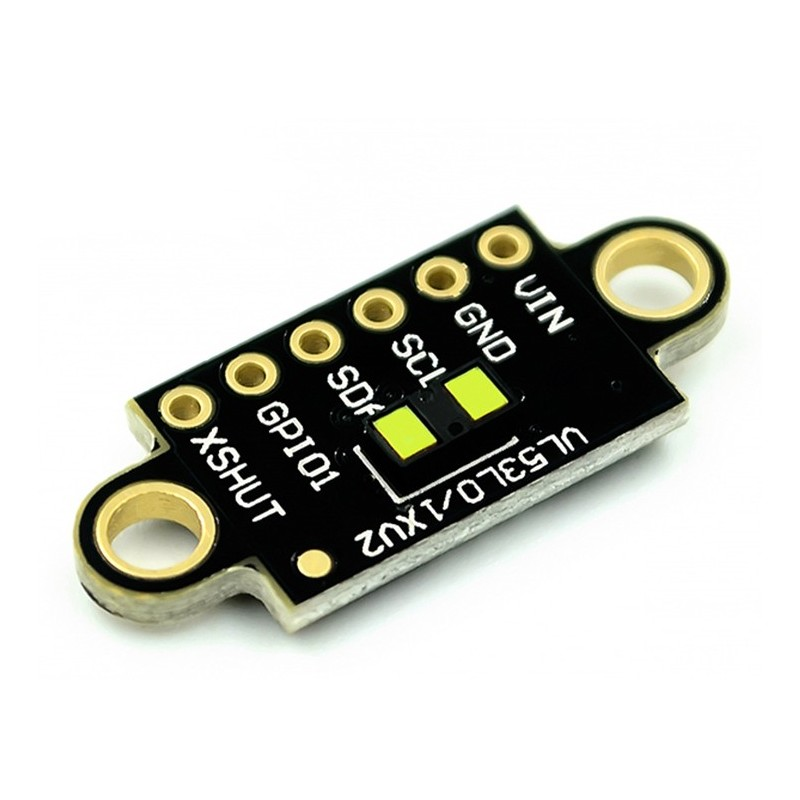
\includegraphics[width=7cm]{includes/images/vl53l1x.jpg}
    \caption{Vzdialenostný senzor VL53L1X}
    \label{fig:vl53l1x}
\end{figure}

Na meranie vzdialenosti sme využili štyri takéto moduly pripevnené na dosku vyosené relatívne od dopredného smeru myši o 45° a 10°.

Z hárdverovej stránky sme potrebovali v tomto projekte vytvoriť dosku plošných spojov (PCB - Printed Circuit Boards) a návrh držiakov motorov, gyroskopu a kolies, ktorých výroba prebiehala pomocou 3D tlače.
\subsection{PCB}
\begin{itemize}
    \item \textbf{Senzory ToF (VL53L1X)}: Prepojenie s ESP32 cez I2C alebo UART rozhranie.
    \item \textbf{Gyroskop s akcelerometrom (MPU9250)}: Prepojenie s ESP32 cez I2C rozhranie.
    \item \textbf{Driver na motor (TB6612FNG)}: Umiestnený blízko motorov, prepojenie s ESP32 cez PWM signály.
    \item \textbf{MCU (ESP32)}: Centrálny riadiaci prvok PCB.
    \item \textbf{Step-up menič na 5V}: Zabezpečenie stabilných 5V pre logické obvody a enkodéry.
    \item \textbf{Logic shifter}: Prekladanie signálov medzi 3,3V a 5V úrovňami.
    \item \textbf{Ochrana batérie}: Meranie napätia batérie a prúdové ochrany.
    \item \textbf{Batéria (Li-ion 1000mAh)}: Umiestnená na PCB s prístupnými napájacími konektormi a ochrannými obvodmi.
\end{itemize}

\textbf{Proces tvorby PCB}
\begin{itemize}

\item \textbf{Návrh schémy}\\
Vytvorili sme detailný návrh elektrickej schémy s prepojeniami všetkých komponentov, pričom sme zabezpečili správne napäťové úrovne a prepojenia medzi jednotlivými časťami.

\item \textbf{Rozmiestnenie komponentov}\\
Strategicky sme umiestnili všetky komponenty na PCB tak, aby boli minimalizované rušenia a zohľadnené fyzické rozmery a montážne obmedzenia.

\item \textbf{Vedenie ciest}\\
Navrhnli sme cesty (trasy) pre prepojenie komponentov, s dôrazom na minimalizáciu kríženia ciest a optimalizáciu pre rušenie (napr. použitie samostatných zemných a napájacích rovín).

\item \textbf{Napájanie a ochrany}\\
Implementovali sme obvody na stabilizáciu napätia (3,3V a 5V), ochrany batérie, a zabezpečili, aby boli všetky komponenty správne napájané a chránené.
 
\end{itemize}

\textbf{Taktiež sme museli myslieť na nasledovné:}
\begin{itemize}
    \item Udržanie minimálnej dĺžky kritických signálových trás (I2C, PWM).
    \item Oddelenie silových a signálových ciest na PCB, aby sa minimalizovalo rušenie.
    \item Zabezpečenie dostatočnej kapacity a filtrácie na napájacích cestách.
    \item Implementácia ochranných obvodov pre batériu a citlivé komponenty.
\end{itemize}

\begin{figure}[!htpb]
    \centering
    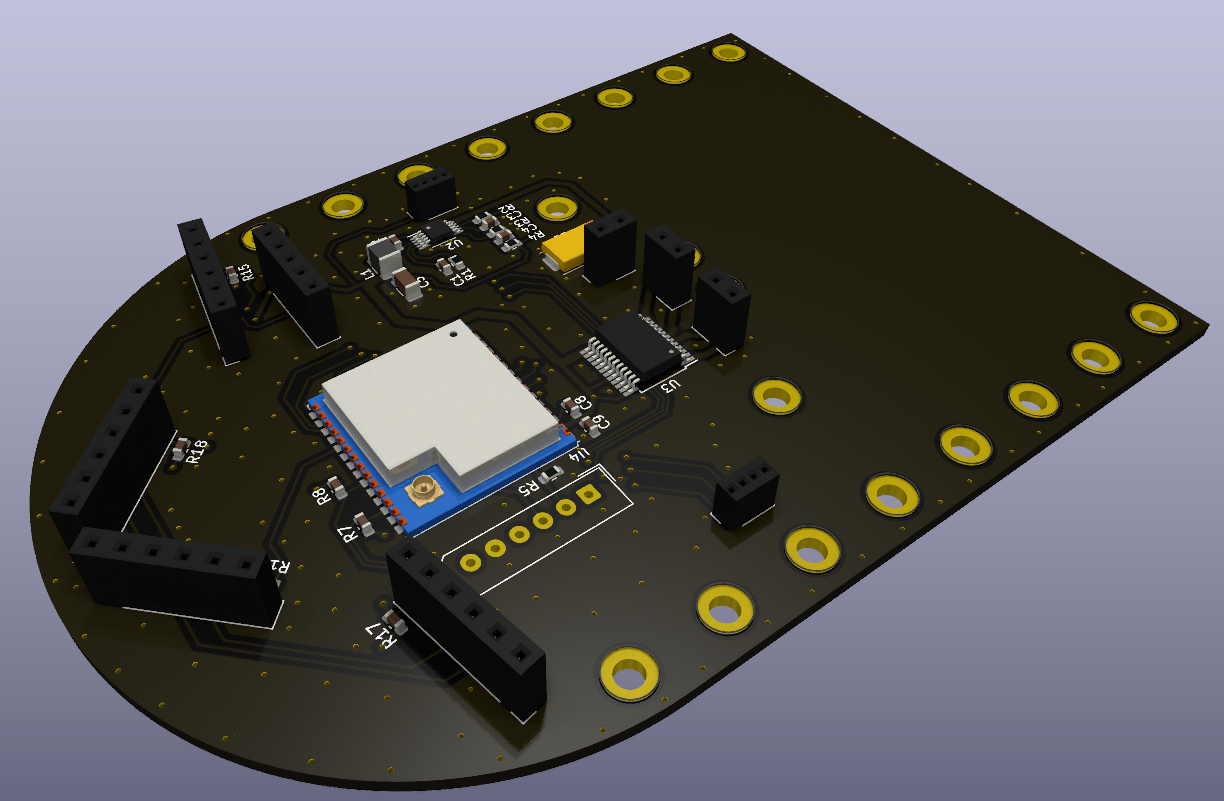
\includegraphics[width=1\linewidth]{includes//images/PCB.png}
    \caption{Návrh PCB dosky použitej vo finálnej verzii.}
    \label{fig:PCB}
\end{figure}

\clearpage\subsection{CAD}
Pri návrhu ako aj pri postupnom iterovaní sme zohľadňovali mnohé aspekty spojené s procesom pri prototypizovaní. Mnohé verzie boli navrhnuté rovnako no v konečnom dôsledku nám ich proces tlače zmenil a museli sme sa s tým vysporiadať, pretože presnosť pri našom návrhu zohrávala kľúčovú úlohu. Pri tlači sme používali dva typy 3D tlače, klasickú FDA no aj živicovú SLA tlač.
\begin{itemize}
\item \textbf{3D návrh kolies}\\
Kolesá pre Micro Mouse boli navrhnuté na základe existujúcich modelov, ktoré poskytli osvedčený základ pre dizajn. Použitie osvedčených modelov umožnilo urýchliť návrhový proces a zaručilo, že výsledné kolesá budú spĺňať požadované špecifikácie.

\item \textbf{Výber modelu}\\
Pre návrh kolies sme vybrali modely, ktoré sú už overené v praxi. Tento prístup minimalizoval riziko návrhových chýb a zabezpečil, že kolesá budú mať vhodné mechanické vlastnosti a správne rozmery.

\item \textbf{Návrh gumy na kolesá}\\
Gumy na kolesá boli použité z existujúceho modelu, čo zabezpečilo optimálnu trakciu a odolnosť. Tento krok eliminoval potrebu vlastného návrhu gumy a umožnil nám sústrediť sa na integráciu kolies do celkového návrhu Micro Mouse.

\item \textbf{3D návrh úchytov}\\
Pre návrh úchytov sme využili iteratívny proces, ktorý umožnil presné prispôsobenie vzdialeností kolies a ich optimálne umiestnenie na Micro Mouse.

\item \textbf{Iteratívny proces návrhu}\\
Návrh úchytov prebiehal v niekoľkých iteráciách, pričom sme upravovali vzdialenosti kolies a ich polohu, aby sme dosiahli najlepšiu možnú stabilitu a pohyblivosť Micro Mouse. Tento proces zahŕňal testovanie rôznych konfigurácií a úpravou návrhu na základe výsledkov týchto testov.

\item \textbf{Optimalizácia vzdialeností}\\
Upravovanie vzdialeností kolies bolo kľúčové pre dosiahnutie optimálnej manévrovateľnosti. Iteratívne úpravy umožnili presné doladenie návrhu, čo viedlo k zlepšeniu celkového výkonu Micro Mouse.
\end{itemize}
\clearpage Návrh a výroba 3D komponentov pre Micro Mouse zahŕňala použitie existujúcich modelov kolies a gumy, ako aj iteratívny návrh úchytov. Tento prístup umožnil efektívne vytvorenie funkčných a spoľahlivých komponentov, ktoré prispievajú k optimálnemu výkonu Micro Mouse.

\begin{figure}[!htpb]
    \centering
    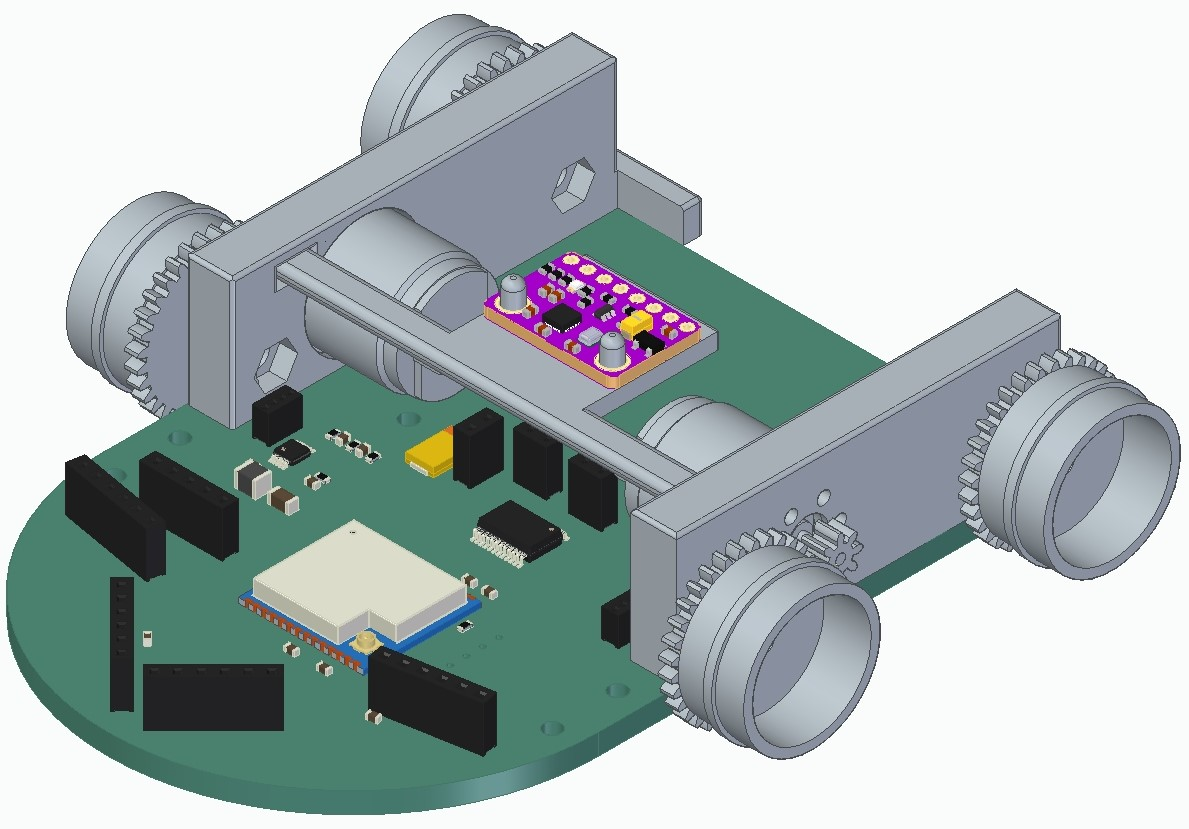
\includegraphics[width=1\linewidth]{includes//images/main_board.jpg}
    \caption{Konečná verzia návrhu všetkých komponentov vyrábaných pomocou 3D tlače usporiadaných na PCB.}
    \label{fig:MainBoard}
\end{figure}

\section{Software}
\label{sec:software}

Na písanie kódu sme použili prostredie \textbf{esp\_idf} verzie \textit{4\.4\.7}, ktoré sme vytvorili za~pomoci
ich repozitára \cite{espGithub}.

Postup na~inicializáciu ESP IDF a~následné spustenie projektu je nasledovný:
\begin{enumerate}
	\item Stiahnutie ESP IDF z~repozitára \cite{espGithub} (My sme použili verziu 4.4.7).
	\item Spustenie príkazu \textit{./install.sh esp32} pre~Linux.
		Tento príkaz stiahne a~nainštaluje všetky potrebne závislosti.
	\item Exportovanie súboru \textit{. ./export.sh} pre~Linux.
		Tento príkaz nastaví všetky potrebne premenne prostredia.
	\item Zmeniť aktuálny adresár na~náš projekt.
	\item Spustiť príkaz \textit{idf.py build} pre~kompiláciu projektu.
	\item Spustiť príkaz \textit{idf.py -P <PORT\_NR> flash} pre~nahratie binárneho súboru do~ESP32.
		Pre tuto operáciu je potrebne mať pripojený počítač a~misku cez UART.
	\item Spustiť príkaz \textit{idf.py monitor} pre~sledovanie výstupu z~ESP32.
\end{enumerate}

Alternatívne spustenie je možné pomocou platformy \textbf{Visual Studio Code} s~nainštalovaným rozšírením
\textbf{ESP-IDF}~\cite{espIDF}.
\subsection{UDP Komunikácia}
Pre spolahlivejšie ladenie a sledovanie správania programu sme implementovali UDP komunikáciu v prostredí Qt Creator v jazyku C++. Táto komunikácia nám umožnila používať realtime grafy na sledovanie správania mikromyši. Súčasťou implementácie bolo aj vytvorenie servera a komunikácia medzi PCB mikromyši a serverom. V tejto komunikácii funguje ESP32 ako klient a počítač ako server. ESP32 posiela údaje o stave mikromyši na počítač, ktorý ich zobrazuje v našej mini HMI aplikácii. 
\begin{figure}[!htpb]
    \centering
    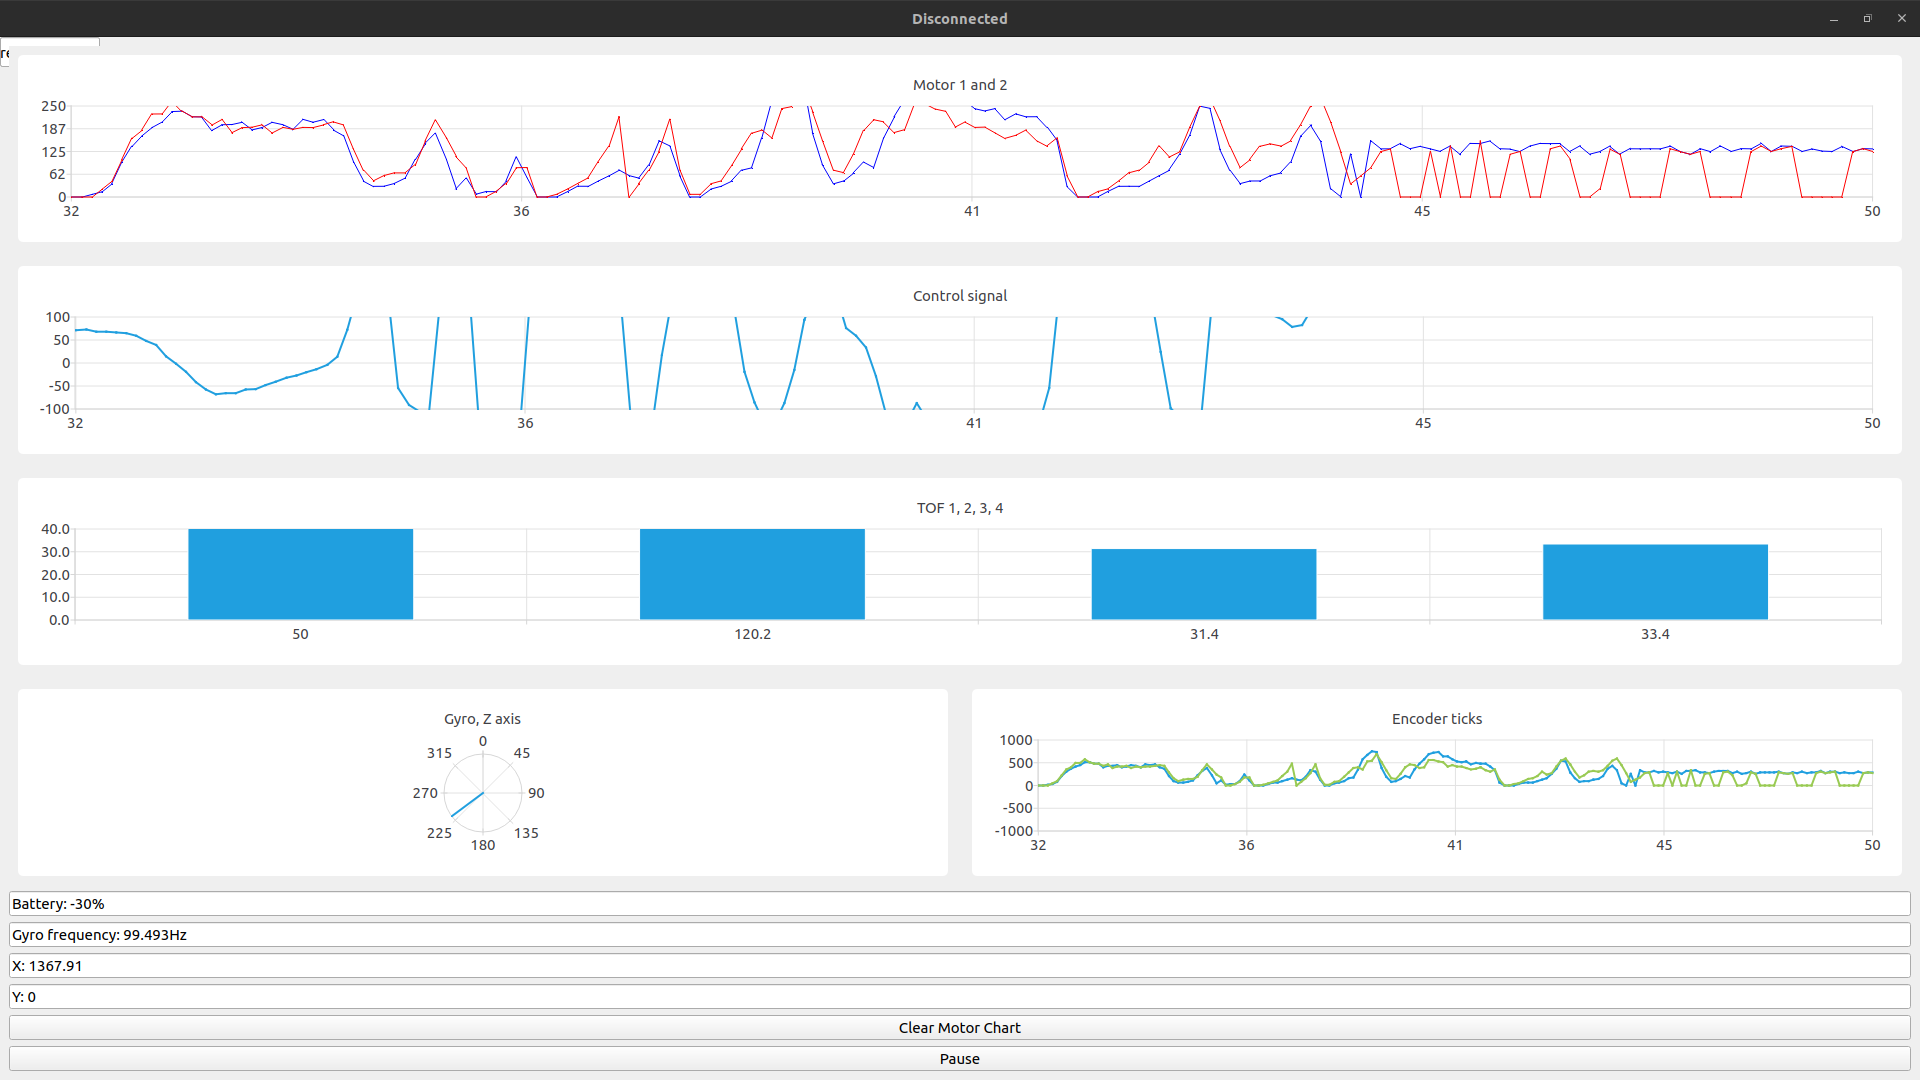
\includegraphics[width=1\linewidth]{includes//images/image.png}
    \caption{Používateľské rozhranie HMI aplikácie }
    \label{fig:UDP}
\end{figure}
Táto aplikácia nám poskytuje efektívny nástroj na ladenie a prácu s mikromyšou, čo nám umožňuje rýchlo a presne reagovať na zmeny a optimalizovať výkon našej autonómnej myšky. \ref{fig:UDP} 
\newpage
\subsection{Senzory}

\subsubsection{VL53L1X}
Pre snímanie vzdialenosti bola vytvorená knižnica na kalibráciu a vyčítavanie dát zo senzora VL53L1X. Komunikácia prebieha prostredníctvom komunikačného protokolu $I^2 C$. Knižnica je nadstavbou nad voľne dostupným rozhraním od STMicroelectronics.

\subsubsection{MPU9250}
\begin{figure}[!htpb]
    \centering
    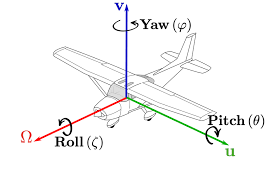
\includegraphics[width=1\linewidth]{includes//images/rpy.png}
    \caption{Gyroskop s akcelerometrom MPU9250 }
    \label{fig:UDP}
\end{figure}
V našom projekte sme použili senzor MPU9250, ktorý je trojosovým akcelerometrom a gyroskopom. Tento senzor nám umožňuje získavať presné údaje o orientácii mikromyši v trojrozmernom priestore. Kľúčovou súčasťou spracovania dát z tohto senzoru je výpočet Eulerových uhlov -- roll, pitch a yaw. Tieto údaje sú neoceniteľné pre stabilizáciu a presné navigačné manévre mikromyši, poskytujúc tak lepší prehľad o jej aktuálnom náklone a orientácii.

\subsection{Odometria}
\label{subsec:odometria}

% Pridat referencia na~motor a~enkoder ked budu vytvorene v~hardweri
Podobne ako v~predmete \textit{Riadenie mobilných robotov} sme použili odometriu na~výpočet polohy robota.
Použili sme na~to inkrementálny enkóder, ktorý je pripojený na~motor. Z enkóderov si získame aktuálnu polohu robota
cez základný vzťah:

\begin{equation}
	\label{eq:odometria}
	 \Delta x_t = x_{t-1} + \Delta s_t \cdot \cos(\theta_{t-1} + \Delta \theta_t)
\end{equation}
\begin{align*}
	\Delta y_t = y_{t-1} + \Delta s_t \cdot \sin(\theta_{t-1} + \Delta \theta_t)
\end{align*}

\newpage

\subsection{PID}
\label{subsec:pid}

Do motorov posielame ako akčný zásah signál PWM (\acrlong{PWM}). Tento signál môže nadobúdať hodnoty od~0 po~1023.
Zároveň musíme myslieť aj na~prepäťovú ochranu. Keď pošleme do~motorov veľké zrýchlenie, tak sa stane, že sa program
na~čipe zresetuje.

Aby sme ošetrili tieto situácie, tak sme neimplementovali PID regulátor s~antiwindup zapojením. Jeho obmedzenie je
nastavené zdola na~0 a~zhora na~1023. Toto obmedzenie zdola je nastavené na~0 kvôli implementácii nastavenia smeru
otáčania motorov. V~prostredí ESP musíme dopredu nastaviť smer otáčania motorov. Po jeho nastavení sa všetky hodnoty
posielajú ako \textit{unsigned}. Teda ak by sme mu poslali zápornú hodnotu, tak by sa motor rozbehol nastaveným smerom.
Antiwindup zapojenie by maximálnu rýchlosť obmedzilo na~1023.

Pre jednoduchosť ovládania sme nastavili regulátor tak, aby vstupná žiadaná hodnota bol v~milimetroch za~sekundu.
Regulátor si túto hodnotu prepočíta na~PWM signál, ktorý pošle motorom. Spätné väzby sa získavajú z~enkóderov
a~dopočítavajú sa na~milimetre za~sekundu. Tieto hodnoty sa taktiež prepočítajú na~PWM signál. Prepočet z~milimetrov
za sekundu na~PWM signál je závislý uskutočňovaný nasledujúcim výpočtom:

\begin{equation}
	\text{PWM} = d \pi \frac{IMP_t}{IMP_{pr} i \Delta t}
	\label{eq:mmps2pwm}
\end{equation}

Rovnica \ref{eq:mmps2pwm} obsahuje parametre:
\begin{itemize}
	\item d - Priemer kolesa,
	\item $IMP_t$ - Aktuálne impulzy z~enkóderu,
	\item $IMP_{pr}$ - Impulzy z~enkóderu za~jednu otáčku (per rotation),
	\item i - Pomer prevodovky motora. Na~našich motoroch je to prevod 32:8,
	\item $\Delta t$ - Časový interval od~posledného merania
\end{itemize}

